\Chapter{Megvalósítás}

Ebben a fejezetben kerül részletes bemutatásra a program implementációjának folyamata. Itt vannak leírva a felhasznált technológiák, nehézségek, érdekesebb problémák és megoldásaik. A fejezet olyan technológiákat is ismertet, amik a program működésének hátterét biztosítják, de konkrét példa nincs rájuk.

\begin{figure}[h]
\centering
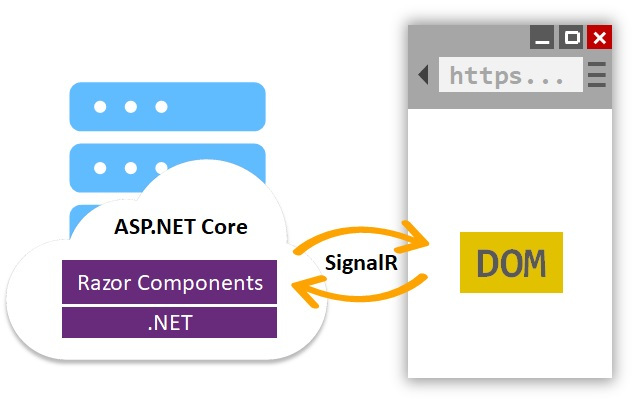
\includegraphics[scale=0.5]{images/blazor.jpg}
\caption{Blazor Server. \cite{blazor}}
\label{fig:blazor}
\end{figure}

\Section{ASP.NET Core Blazor}
A megvalósításra felhasznált technológia végül a \textit{ASP.NET Core Blazor}  \cite{blazor} lett, ami egy .Net \cite{dotnet} keretrendszer komplex, interaktív webalkalmazások létrehozására. Lényege, hogy a weboldalhoz  JavaScript \cite{js} helyett C\# \cite{csharp} kódot írhassunk. Kicsit pontosabban, szinte minden frontend logikához C\# kód a megoldás HTML elemek elrendezésétől a weboldal navigálásán át fájlok feltöltéséig.

Jelenleg 2 verziója támogatott, a \textit{Blazor Server}  \cite{blazor_h} ahol egy szerver alkalmazásban fut a kód (\ref{fig:blazor} ábra), és a \textit{Blazor WebAssembly} \cite{blazor_h}, ahol közvetlenül a böngészőben. Ebben a projektben a \textit{Blazor Server}-t választottam a nagyobb támogatottsága miatt.

\Section{Razor komponensek}
Blazor alkalmazások jelentős részben \textit{Razor} komponensekből épülnek fel \cite{razor}. Egy komponens az UI egy önálló része, ami tartalmazhat feldolgozó logikát, hogy dinamikusan viselkedhessen. Komponenseket lehet többször felhasználni, egymásba ágyazni, vagy Razor oldalakban felhasználni (egy komponens akár önmagában is lehet Razor oldal). Egy Razor komponens tartalmaz HTML elemeket és @ jellel ellátott C\# kifejezéseket, amik lehetnek direktívák, logikák, vagy akár komplex kódrészek is.

\Section{Routing, SignalR, és Dependency Injection}
A routing, azaz útvonal választás, az a folyamat, ahogy a szerver a bejövő HTTP kéréseket az alkalmazás végrehajtható végpontjaihoz párosítja. Az ASP.Net ezt szinte automatikusan teszi meg, a megfelelő kérést a megfelelő Razor oldalra irányítja, miután megadjuk neki a kellő navigációs beállítást. Navigációs beállítás lehet például autentikáció.

Viszont nem minden interakció eredményez HTTP kérést, a legtöbb kommunikáció a weboldal és a szerver között SignalR segítségével történik \cite{signalr}. A SignalR egy nyílt forrású könyvtár, ami lehetővé teszi a valós idejű kommunikációt a szerver és a weboldal között. Ha a UI egy interaktív elemét "megpiszkájuk", a weboldal SignalR-en át átküldi az esemény(eke)t a szervernek, a szerver végrehajtja a kérést, majd szintén SignalR-en keresztül visszaküldi a UI frissítéseket.

A \textit{Dependency Injection} \cite{di} egy szoftver fejlesztési technika, aminek lényege, hogy megfordítja az irányítást elemek és függőségeik között. ASP.NET-ben ez annyit jelent, hogy az osztályok vagy komponensek ahelyett, hogy önmaguk hoznák létre vagy konstruktorukban kapják meg a függőségeiket, egy úgynevezett DI konténer hozza őket létre. 3 féle módon lehet a függőségeket kezelni.	
\begin{itemize}
\item\textbf{Transient Object:} Minden esetben új és egyedi objektumot hoz létre.
\item\textbf{Scoped Object:} Egy kérésen belül ugyanazt az objektumot biztosítja.
\item\textbf{Singleton Object:} Minden esetben ugyanaz a (meglévő) objektum.
\end{itemize}
Ez az alkalmazás főleg \textit{Singleton}-okat használ szolgáltatások biztosítására és közös adatok elérésére. Mivel végig egy felhasználó dolgozik egy munkamenetben, nincs szükség limitálni a függőségek élettartamát és elérhetőségét.

Singleton regisztrálása a program.cs-ben.
\begin{cpp}
builder.Services.AddSingleton<MyFile>();
builder.Services.AddSingleton<MockInstructionList>();
builder.Services.AddSingleton<MenuService>();
\end{cpp}

Dependency Injection használata a Simulation.razor-ban.
\begin{cpp}
@page "/simulation"
@inject Models.MyFile myFile
@inject Services.DebugService debugService;
@inject Services.ImageService imageService;
@inject Services.Analysis analysis;
\end{cpp}

\Section{Fájlok feltöltése}
Fájl feltöltéséhez nincs külön \textit{Service} osztály, hanem minden az \textit{UploadFile	 Razor} komponensben zajlik. A tényleges feltöltést egy beépített \textit{InputFile Razor} komponens végzi \cite{upload}. A fájl feltöltése után a fájl sorokra van bontva, majd átkerül a perzisztens objektumhoz, ahonnan más oldalak el tudják érni. Ezután meghívásra kerülnek a különböző elemző, szimuláló és vizualizáló szolgáltatások (\ref{fig:up} ábra).

\begin{figure}[h]
\centering
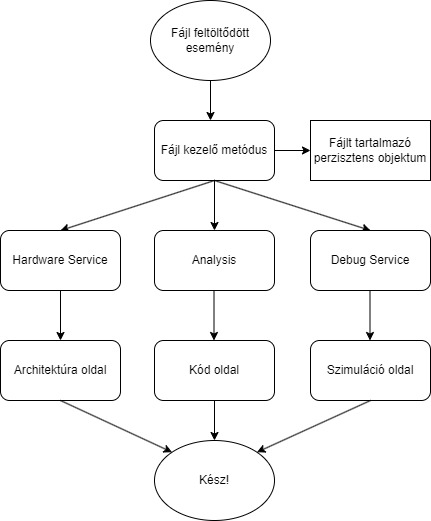
\includegraphics[scale=0.8]{images/UploadFlow.jpg}
\caption{Feltöltést követő folyamatok.}
\label{fig:up}
\end{figure}

\Section{Hardware Service}
A .NET Core hivatalosan egy multiplatform alkalmazás, de sajnos még vannak olyan részei amik jelenleg még csak a Windows-t támogatják. A Hardware elemzésére a hivatalosan támogatott módszer a WMI (\textit{Windows Management Instrumentation}) használata, nevéből adódóan jelenleg csak Windows-on elérhető, ezért más operációs rendszerek esetében az alkalmazás hamis, kitalált adatokkal dolgozik, amíg a Microsoft ki nem terjeszti a támogatását Linuxra és társaira. Ahogy \aref{fig:hws} ábra mutatja, a WMI-ből szerzett információkat Dependency Injection juttatja el a frontenthez.

\begin{figure}[h]
\centering
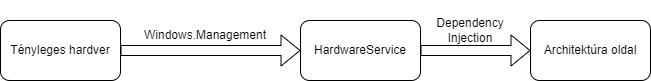
\includegraphics[width=\textwidth]{images/HWS.jpg}
\caption{Hardware Service.}
\label{fig:hws}
\end{figure}

Proceszzor management objektum megszerzése.
\begin{cpp}
ManagementObject CPU = 
	new ManagementObjectSearcher("select * from Win32_Processor")
            .Get()
            .Cast<ManagementObject>()
            .First();
\end{cpp}

\Section{Navigation Menu}
Az alkalmazásban a navigáció különböző oldalak között az oldalsó navigációs menün keresztül történik. Ennek az az érdekessége, hogy a menüpontok csak akkor jelennek meg, ha tartalmuk készen áll. Itt olyan probléma merült fel, hogy a menü nem frissül magától, ezért be kellett iktatni egy új szolgáltatót, a \textit{MenuService}-t. A \textit{MenuService} feladata egy esemény kezelése. Ha a programban olyan változás történik, ami hatással van a menüre, a szolgáltatás meghívja az eseményt, amit a menü már észlelni tud és lereagálja (\ref{fig:MenuEvent} ábra). 

\begin{figure}[h]
\centering
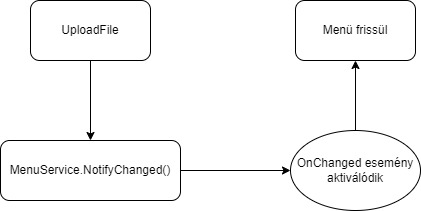
\includegraphics[scale=0.8]{images/MenuS.jpg}
\caption{Frissítési esemény működése.}
\label{fig:MenuEvent}
\end{figure}

\Section{Architeture oldal}
Az Architecture oldal fő és egyetlen eleme egy \textit{Canvas}, pontosabban egy \textit{Blazor Extension Canvas}, ami azért előnyös, mert könnyen manipulálható C\# kóddal. Ez a komponens miután létrehozza a \textit{Canvas}-t, megrajzolja a \textit{Hardware Service} által szolgáltatott adatokat, mint a fizikai memória, CPU, GPU. Az egyszerűség kedvéért fix méretű \textit{Canvas}-al dolgozik, így pixel pontosan meg tudja rajzolni az entitásokat és a kapcsolatokat.

\Section{Analysis}
Ez az egyik fő alkotóeleme a programnak. Itt megvizsgáljuk a beolvasott fájlt, és sorról sorra végigmegyünk rajta OpenCL elemeket kutatva. 

Első lépésben megvizsgálja, hogy a program CPU-nak vagy GPU-n fut-e, és ez alapján megállapítja a megfelelő \textit{Compute Unit} mennyiséget, ami processzor esetén a logikai szálakkal egyenértékű. Viszont videokártya esetén ez egy sokkal összetettebb probléma, nem lehet ilyen egyszerűen megmondani a számítási egységek mennyiségét. Például egy NVIDIA GeForce GTX 1080 videókártyában 2560 CUDA mag, 160 texture mapping unit, és 64 ROP egység található \cite{1080}. Ez egyrészt nem látható a WMI számára \cite{wmi}, másrészt ebből kikövetkezthetetlen a tényleges OpenCL számítási egységek száma. Ettől csak bonyolultabb esetek vannak. Lehetnek Tensor \cite{tensor} magok is, lehet integrált videókártya ami bizonyos erőforrásokon a processzorral osztozik, más gyártású, például AMD videókártyák pedig teljesen más felépítésűek is lehetnek. Ha sikerülne is megállapítani a számítási egységek számát, 3000+ számítási szálat nem lehet jól vizualizálni, ezért videókártya esetén az ábrázolás céljából a program egy kitalált 4 számítási egységgel fog dolgozni.

Második lépésben összegyűjti az OpenCL elemeket egy listában és megadja a hozzájuk tartozó számítási egység számát. Ez lehet:
\begin{itemize}
\item\textbf{0:}  ami azt jelenti hogy egy szálon fut szekvenciálisan,
\item\textbf{1, 2, 3, $\ldots$:}  ami a hozzá tartozó tényleges számítási egység száma,
\item\textbf{-1:}  ami azt jelöli, hogy az összes elérhető számítási egységen párhuzamosan történik.
\end{itemize}

\Section{Code oldal}



Ez a második megjelenítő felület (\ref{fig:code_plan} ábra). 2 egymás mellett lévő konténerből épül fel.
A baloldali konténerben egy dinamikus táblázat foglal helyet, ami a már elemzett objektumokat jeleníti meg Gannt diagram formában. A diagram bal oldalán a végrehajtás lépésének indexe, tetején pedig a számítási egységek sorszámai szerepelnek, plusz a 0-s oszlop ami a szekvenciális futást jelzi. A diagram a számítási egységeknek megfelelően az oldal betöltésekor dinamikusan töltődik fel elemekkel. A diagram elemei HTML gombok, amik tartalmazzák az elemek neveit, valamint a megfelelő funkciókat. Szükséges a ciklusváltozó "elfogása" az ii változó által, ellenkező esetben a függvények mindannyian az alap ciklusváltozó végső értékét fogják használni.

\begin{cpp}
@for(int i = 0; i < Analyzer.myElements.Count; i++)
 {
   int ii = i;
   <tr>
      <td>@(i+1)</td>
      @for(int j = 0; j < Analyzer.CUs + 1; j++)
        {
          <td style="min-width:50px">
          @if (j == Analyzer.myElements[ii].ComputeUnit | (j != 0 &
               -1 == Analyzer.myElements[ii].ComputeUnit))
             {
                <button title=@Analyzer.myElements[ii].Name @onclick="()
                =>{ChangeColor(Analyzer.myElements[ii].Index);ScrollTo
                Analyzer.myElements[ii].Index);}">@(i+1)</button>
             }
          </td>
        }
   </tr>
 }
\end{cpp}

\begin{figure}[h]
\centering
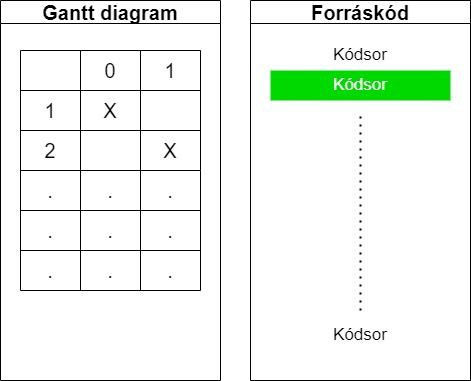
\includegraphics[scale=0.5]{images/Code_plan.jpg}
\caption{Code oldal felülete.}
\label{fig:code_plan}
\end{figure}

A második konténerben, vagyis az oldal jobb oldalán, magát a forráskódot jelenítjük meg sorokra osztva, az üres sorokat még a feldolgozás közben eltávolítva. Minden sor külön paragrafus elem, \textit{id}-val ellátva, hogy lehessen rájuk hivatkozni. Itt lesz szerepe a Gannt diagram gombjainak. Egy gomb megnyomásakor a hozzá tartozó elem színe zöldre, a többi pedig fehérre vált. Ez a fent említett \textit{SignalR}-en keresztül zajlik, majd ugyanitt frissül az oldal, és a megfelelő kódsor paragrafusa ténylegesen zöldre vált. Emellett a böngésző a megfelelő helyre is teker, ami JavaScript-et igényel. A program ekkor \textit{JavaScript Interop} használatával meghív egy JS függvényt (\ref{fig:jspl} ábra), ami elvégzi a kérést \cite{js_interop}.



\begin{figure}[h]
\centering
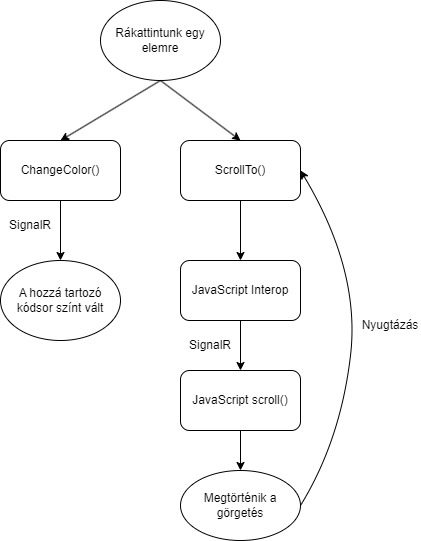
\includegraphics[scale=0.85]{images/JSpl.jpg}
\caption{\textit{JavaScript InterOp SignalR}-n át.}
\label{fig:jspl}
\end{figure}

\begin{cpp}
jsRuntime.InvokeAsync<bool>("test", "line{" + (i-8) + "}");
\end{cpp}

\newpage

\Section{Instrukciók és szimulálásuk}
A program az átmeneti kódot instrukció objektumonként kezeli, ami az instrukció típus \textit{enum}-ból és különböző adattagokból áll. Az adattagoknak a típusaikon (\textit{string, int, double}) túl nincs kötött szerepe, hanem az instrukció kezelő szükség szerint használja őket. A \ref{tab:instru} táblázat bemutat implementált instrukciókat és hozzájuk tartozó kezelő metódusokat. Az összes adattag nullázható típus, ami szükséges az instrukciók korrekt létrehozásához és működéséhez, viszont bonyolítja kezelésüket.

\begin{table}[h!]
\centering
\caption{Implementált Instrukciók és hozzájuk tartozó szimuláló metódusok}
\label{tab:instru}
\begin{tabular}{|c|c|}
\hline
DECLARE (array) & Create(array)Type(), CreateArray(), AssignValue()  \\
\hline
COPY (tömbökkel) & COPY(ToArray)(FromArray)(ToArrayFromArray)() \\
\hline
UOP (tömbökkel) & UOP(ToArray)(FromArray)(ToArrayFromArray)() \\
\hline
JUMP (feltétellel) & Jump() (feltételekkel)\\
\hline 
PRINT (tömb) & Print() (tömb) \\
\hline
PARALLEL & Start és End metódusok \\
\hline
Barrier & nincs külön kezelő metódus \\
\hline
\end{tabular}
\end{table}

Az instrukciók 2 féle módon jönnek létre, vagy hamisak és "kitalálja" őket a program a forrásfájl neve alapján, vagy a felhasználó adja meg őket. Az első esetben egy \textit{MockInstructionList} objektum hozza őket létre, második esetben pedig egy \textit{InstructionParser} objektum, de egyaránt egy \textit{MockInstructionList} objektumban lesznek eltárolva egy listában.

\begin{cpp}
public MockInstructionList ParseInstructons(string textInstructions)
{
    String[] textInstructionArray = textInstructions.Split('|');
    MockInstructionList list = new MockInstructionList();
    foreach(String instruction in textInstructionArray)
    {         
        list._instructions.Add(ParseInstruction(instruction));
    }
    return list;
}
        
private Instruction ParseInstruction(string textInstruction)
{
    ......
    return  new Instruction
	(
		parseInstructionType(instructionType[1]),
        nullCheck(currentInstructionArray[1]),
        nullCheck(currentInstructionArray[2]),
        nullCheck(currentInstructionArray[3]), 
        nullCheckInt(currentInstructionArray[4]),
        nullCheckDouble(currentInstructionArray[5]),
        nullCheckDouble(currentInstructionArray[6]),
        instructionVar7,
        instructionVar8
	);
}
\end{cpp}





Ezután az instrukciók átkerülnek a \textit{DebugService}-hez, ahol megtörténik a szimuláció.
A \ref{fig:debugflow} ábra egyszerűsített módon illusztrálja a a szimuláció működését. A szimuláció első lépése a változók és tömbök létrehozása és tárolása. Mivel nem lehet előre tudni a változók neveit, típusait, mennyiségeket, dinamikus megoldásra van szükség. Ilyen lehetett volna változó és tömb listák, és a hozzájuk tartozó szótárak létrehozása. Változó létrehozásakor hozzáadódna listához, majd bekerülne a szótárba, mint egy \textit{<változó név,index>} elempár, és a szótáron át lehetne rá hivatkozni. Működőképes, de komplikált és problémás, mivel a szótár egy extra réteg az adatok és az instrukció kezelő között. Minden adattípushoz külön \textit{lista - szótár} páros lenne szükséges, tömb listák is bonyolítanák.

\begin{figure}[h]
\centering
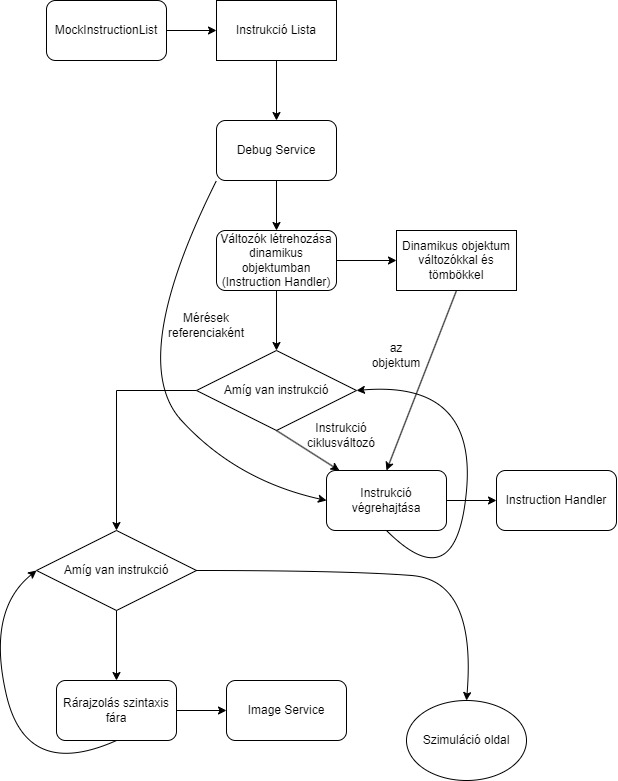
\includegraphics[scale=0.65]{images/SimpleDebug.jpg}
\caption{A \textit{Debug Service} egyszerűsített folyamatábrája.}
\label{fig:debugflow}
\end{figure}



A megoldás egyszerre bonyolultabb és egyszerűbb. Futásidőben hozunk létre egy osztályt a szükséges adattagokkal. Ehhez felhasználjuk a \textit{Reflection} \cite{reflection} könyvtárat, főleg az \textit{AssemblyBuilder}-t, \textit{ModelBuilder}-t, és a \textit{TypeBuilder}-t \cite{assembly_builder}. Ezek létrehozzák az osztályt, majd az instrukciók kezelő létrehozza a megfelelő mezőket, amik lehetnek \textit{string} vagy \textit{double} változók, vagy tömbök. Az instrukció kezelő az instrukció típusa alapján hívja meg a korrekt metódust. Ekkor egyiknek sincs értéke.

\begin{cpp}
AssemblyBuilder assemblyBuilder = 
AssemblyBuilder.DefineDynamicAssembly(...);
ModuleBuilder moduleBuilder = 
assemblyBuilder.DefineDynamicModule(...);
TypeBuilder typeBuilder = moduleBuilder.DefineType(...);
foreach (Instruction instruction in instructions)
{
    instructionHandler.
    ExecuteDeclaration(...);
}


private void CreateType(...)
{
	switch (type)
    {
    	case "string":
        	typeBuilder.DefineField
            (name,typeof(string),FieldAttributes.Public);
            break;
		default:
        	typeBuilder.DefineField
            (name, typeof(double), FieldAttributes.Public);
            break;
    }
}
\end{cpp}

Van lehetőség konstruktorokat is megadni, és úgy adni értékeket a változóknak, de problémát okozhat ha egy tömb méretét egy változó szabná meg, és a változónak még nincs értéke. Ezért a deklarációk után befejeződik az osztály készítése, és létrejön egy példánya.
Az objektum létrehozása után megkezdődik az igazi szimuláció, az összes instrukció feldolgozásra kerül. Ha hivatkozni szeretnénk egy változóra, az objektumon át érjük el reflekció segítségével, az objektum típusának mezőjének értéket tudjuk így egyszerűen elérni.

\begin{cpp}
private string VarPrint(string name, Object object)
{
	return "Value of {name} : 
    {object.GetType().GetField(name).GetValue(object)}";
}
\end{cpp}

Néhány instrukció paramétere lehet érték vagy változó ami értéket tárol. Ilyen esetben az instrukció kezelő dönt.



\begin{cpp}
double opValue;
if (doubleValue.HasValue)
{
    opValue = doubleValue.Value;
}
else
{
     opValue = (double)object.GetType().
     GetField(value).GetValue(object);
}
\end{cpp}

Érdekesség, hogy néha szükséges átváltani az objektum egy \textit{double} elemét \textit{int}-é. Ennek módja általában a \textit{(int)var} -al történik, de az itt hibát okoz a változó ki-be- csomagolása miatt, ezért vagy \textit{(int)(double)var} -t kell használni, vagy \textit{int.convert(var)}-t.

Prédikátumok az átmeneti kódban ugrásokra vannak bontva, ha egy prédikátum teljesül, akkor a szimuláció indexe továbbugrik a megjelölt instrukcióhoz. Elöltesztelő ciklus esetén van egy második ugrás a ciklus végén, ami visszaállítja a szimuláció indexét a ciklushoz tartozó prédikátumhoz.

A futtatás során feljegyzésre kerül az instrukció lépésszám, és a a változók és tömbök által lefoglalt memória igény, ami a program minimum memóriaigényének felel meg, valamint méri a futási időt is. Az analízis segítségével kimutatásra kerül a \textit{local} és \textit{global Size}, illetve a munka csoportok mennyisége is. 



\Section{Párhuzamosság szimulálása}
A szimuláció pontosan követi a szimulált program párhuzamosságát. Egy párhuzamos szakaszt két különleges instrukció, a PARALLEL{\_}START és a PARALLEL{\_}END határol körbe. Az instruction handler a PARALLEL{\_}START instrukciót követve a normál működés helyett az azt követő instrukciókat eltárolja egy saját instrukció listában, amíg el nem éri a PARALLEL{\_}END instrukciót. Ezután az instrukcióban megadott szálakon párhuzamosan végrehajtja az eltárolt instrukciókat, majd visszaállítja a rendes működést (\ref{fig:parallelSim} ábra).


\begin{figure}[h]
\centering
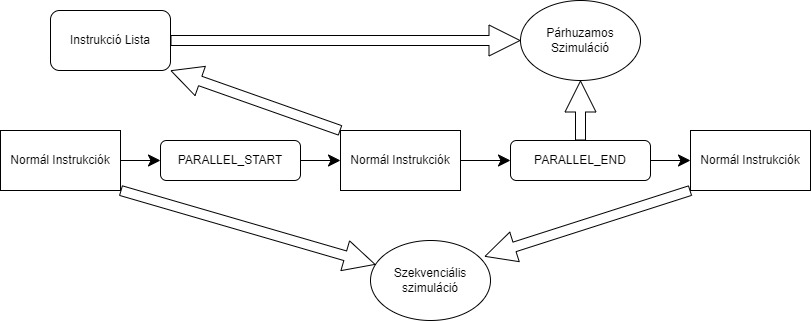
\includegraphics[width=\textwidth]{images/Parallel_Simulation.jpg}
\caption{Párhuzamos szimuláció}
\label{fig:parallelSim}
\end{figure}


A párhuzamos szimuláció a \textit{Parallel.For()} \cite{pfor} metódussal történik, így pontosan annyi párhuzamos folyamatot tudunk indítani, amennyi szükséges. A ciklusban a végrehajtani kívánt utasításokat egy lambda kifejezésben adjuk meg, amiben egy újabb, a párhuzamos instrukciós listán iteráló ciklus végzi el a szimulációt. Ilyenkor az instrukciók a normális index helyett a hozzájuk tartozó folyamat azonosító számmal dolgoznak, ami a létrehozásuk sorrendjének felel meg. Az instrukciós lista egy \textit{Immutable list} objektum, azaz módosíthatatlan. Ennek következménye, hogy a lista csak olvasható lesz, ezért az összes párhuzamos folyamat egy időben el tudja érni, ezzel is gyorsítva a szimulációt.

Implementálásra került a barrier párhuzamos vezérlési utasítás is. A barrier lényege,  hogy egy olyan pont, amit minden párhuzamos szálnak el kell érnie mielőtt bármelyik továbbhaladhat. Ennek C\# megvalósítása a \textit{Barrier} osztály, ami a célnak megfelelt volna, de túlságosan lassúnak bizonyult, ahogy \aref{tab:barrier} táblázaton látható.



\begin{table}[h]
\centering
\caption{Barrier implementációk futási ideje}
\label{tab:barrier}
\begin{tabular}{|c|c|}
\hline
Barrier 20 szálra & 10 sec  \\
\hline
Barrier 40 szálra & 26 sec \\
\hline
Barrier 80 szálra & 67 sec \\
\hline 
Saját barrier 10000 szálra & <1 sec \\
\hline
\end{tabular}
\end{table}

A saját barrier implementáció a \textit{Parallel.For()} metódus egy sajátosságát használja ki. A metódus nem tér vissza amíg az összes általa indított párhuzamos szál véget nem ér. Így egy primitív barrier-ként funkcionál, abban az esetben ha az barrier a párhuzamos instrukciók legvégén van. Ezt kihasználva szét kell szedni az instrukciós listát a BARRIER utasítások alapján, és külön futtatni őket. De ahelyett, hogy ténylegesen szétszednénk több listára, az egész párhuzamos szimulációt egy újabb ciklussal burkoljuk, ami addig tart amíg a párhuzamos szakasz a végére nem ért. A szakasz végét úgy észleljük, hogy a instrukció mutató meghaladja az instrukciók mennyiségét. 

Ezt az instrukció iteráló ciklus indexével mérjük, párhuzamos szálanként külön-külön. Barrier-höz érve véget ér az adott szál, az instrukció mutató változó eltárolódik, majd ha az összes szál befejeződik, véget ér az őket indító \textit{Parallel.For()} metódus. Ezután a barrier-t imitálva elindul a következő instrukció szakasz a következő \textit{Parallel.For()} blokkban az eltárolt instrukció mutatótól kezdve (\ref{fig:Barrier} ábra). 



\begin{cpp}
while (parallelLoop!=parallelCount)
    {
        Parallel.For(0, parallelCount, (i, state) =>
        {
            if (start[i] >= parallelInstructions.Count)
            {
                Interlocked.Increment(ref parallelLoop);
                return;
            } 
            for (int j = start[i]; j < parallelInstructions.Count;)
            {
                if (...instrucionType == ...BARRIER)
                   {
                       j++;
                       start[i] = j;
                       break;
                   }
                ExecuteInstruction(...);
                start[i] = j;
            }
        });
    }
\end{cpp}

\begin{figure}[h]
\centering
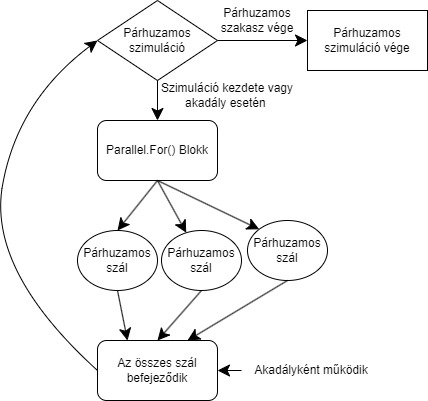
\includegraphics[scale=0.9]{images/Barrier.jpg}
\caption{Barrier implementáció}
\label{fig:Barrier}
\end{figure}

\Section{Szintaxis fa}
A szimuláció után a \textit{DebugService} az \textit{ImageService} segítségével létrehoz egy szintaxis fát, amin fel van tüntetve az összes instrukció, és a hozzájuk tartozó nyilak. A kép egy dinamikusan bővülő \textit{bitmap}-ből készül el, így minimális méretű. Itt két érdekesebb probléma merült fel, az egyikben az alkalmazás lementi a készült képet, majd a böngésző megjeleníti. A kép bővülésének módja \aref{fig:st} ábrán látható. De ha új képre akarunk váltani, a böngésző a régi képet fogja mutatni, mert eltárolta a gyorsítótárban. Így minden kép sorszámot kap, hogy a böngésző észlelje hogy új képre van szükség, és ne a gyorsítótárból szedje elő. 

A másik érdekes probléma a kép dinamikus bővítése közben történt. A képre rárajzolódott minden rendesen, megtörtént az átméretezés, de a tényleges kép a memóriában nem méreteződött át. Olyan, mintha a \textit{bitmap} objektum egyszerre lenne érték és referencia típus, aminek oka ismeretlen. Szerencsére ha explicit módon referencia típusként kezeljük, akkor ez a hiba gyorsan megoldódik.

\begin{cpp}
public Bitmap AddInstruction(ref Bitmap bitmap,String text,bool jump)
{
      if (bitmap.Width > 220)
      {
           DrawRectangleText(bitmap, text, jump);
           DrawStraightArrow(bitmap);
       }
       else
       {
           DrawRectangleText(bitmap, text, jump);
       }
       bitmap = ResizeBitmap(bitmap, 200);
       return bitmap;
}
\end{cpp}

Miután elkészül a szintaxis fa, az alkalmazás elkészíti a szimuláció oldalt, ahol az eredmények láthatóak.

\begin{figure}[h]
\centering
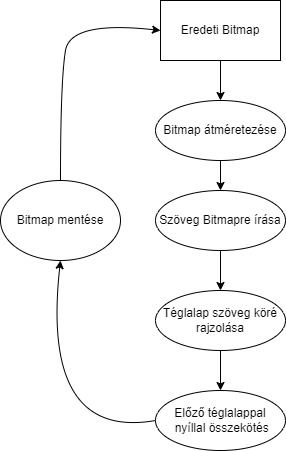
\includegraphics[scale=0.8]{images/ST.jpg}
\caption{Elem hozzáadása a szintaxis fa bitmapjéhez.}
\label{fig:st}
\end{figure}


\Section{Platform függetlenség}
2016-ban megjelent a .Net Core 1.0, ami az addigi .Net keretrendszer platform független verziója lett. A dolgozatban használt .Net 6.0 ennek a legújabb hosszútávú támogatású verziója, ami szintén platform független. A Blazor webalkalmazás szintén platformfüggetlen. Néhány használt könyvtár viszont még nincs  frissítve, ezért Linux-on vagy nem (System.Management-et nem használjuk Linuxon), vagy korlátozottan (System.Drawing.Common-al \cite{drawing})  működik. Az alkalmazás így is platformfüggetlen, de csak Windowson volt tesztelve.

%\begin{verbatim}
%$ some commands with arguments
%1 2 3 4 5
%$ _
%\end{verbatim}


